
\فصل{نتایج تجربی}
\label{sec:results}
‌
در این فصل به بررسی نتایج به دست آمده حاصل از روش پیشنهادی که در فصل گذشته به‌طور مفصل راجع‌به آن صحبت کردیم، می‌پردازیم.

\قسمت{مجموعه دادگان}

در این قسمت مجموعه‌دادگان آموزش و آزمون مدل‌های پیشنهادی معرفی می‌شوند و پیش‌پردازش‌های انجام شده روی هریک آورده شده است.
همان‌طور که در قسمت قبل یعنی مدل پیشنهادی صحبت شد، در آن مدل ما تعدادی شاخص داریم مانند کیفیت کالا.  حال در مجموعه دادگان آموزش اپراتورهای دیجی‌کالا حدود ۲۵ میلیون کامنت را برچسب‌گذاری کرده‌اند و از آن در مدل خود استفاده نموده‌ایم. اندازه‌ی مجموعه دادگان نقش بسیار مهمی در دقت مدل به‌دست آمده دارد.
\قسمت{معیار‌های اندازه‌گیری}

برای اندازه‌گیری دقت مدل، روش‌های گوناگونی وجود دارد که ابتدا سه تا از مهم‌ترین معیارها را معرفی کرده و در قسمت بعدی به مقایسه‌ی نتایج به دست‌آمده از دقت هر کدام از روش‌ها برای همه‌ی شاخص‌ها خواهیم پرداخت.

\begin{itemize}
    \item \textbf{معیار \lr{Precision}}
    برابر است با تقسیم تعداد مواردی که توسط مدل درست تشخیص داده شده‌است بر تعداد مواردی که واقعاً درست هستند، درست تشخیص داده شده‌اند.
    از همین رو فرمول این معیار به شیوه‌ی زیر محاسبه می‌شود.
        \begin{equation}
            recall = \dfrac{true \: positive}{true \: positive + false \: positive}
        \end{equation}
    \item \textbf{معیار \lr{Recall}}
    برابر است با تقسیم تعداد مواردی که توسط مدل درست تشخیص داده‌اند شده بر تعداد کل مواردی که توسط مدل ایجاد شده‌اند. به بیان دیگر از تعداد کل موارد صحیح، چه تعداد را توانسته‌ایم درست حدس بزنیم. از همین رو فرمول این معیار به شیوه‌ی زیر محاسبه می‌شود.
        \begin{equation}
            precision = \dfrac{true \: positive}{true \: positive + false \: negative}
        \end{equation}
    \item \textbf{معیار \lr{F1}}
     در دو مورد قبل، Precision و Recall را معرفی و به صورت دقیق تعریف کردیم. حال معیار 
     \لر{F1 Measure}
     یک نوع میانگین بین این دو است که به شکل زیر محاسبه می‌شود.
     
        \begin{equation}
            F_1 = 2 \times \dfrac{precision \times recall}{precision + recall}
        \end{equation}
\end{itemize}

\قسمت{دقت ‌مدل بر اساس معیارهای متفاوت روی شاخص کیفیت}

\begin{figure}[H]
\centering
\caption{ ‌مدل بر اساس معیارهای متفاوت روی شاخص کیفیت}\label{}
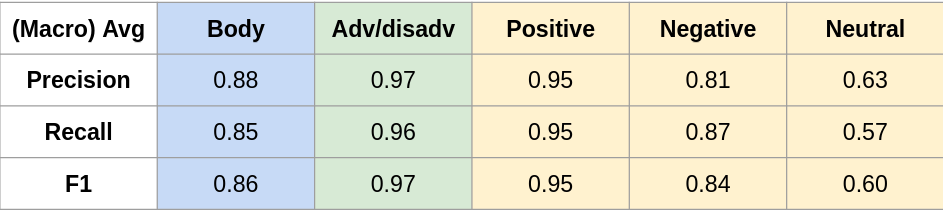
\includegraphics[width=15cm]{figs/quality.png}
\label{fig:test}
\end{figure}


\قسمت{دقت ‌مدل بر اساس معیارهای متفاوت روی شاخص ارزش نسبت به قیمت}
\begin{figure}[H]
\centering
\caption{ ‌مدل بر اساس معیارهای متفاوت روی شاخص ارزش نسبت به قیمت}\label{}
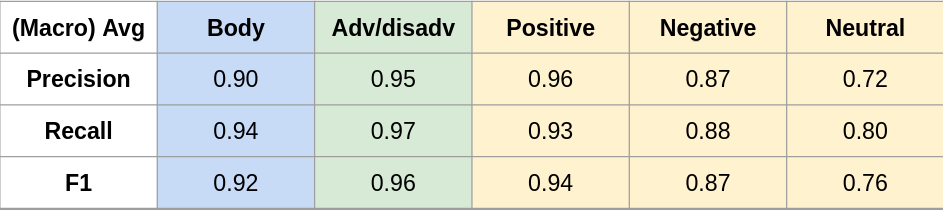
\includegraphics[width=15cm]{figs/price.png}
\label{fig:test}
\end{figure}


\قسمت{دقت ‌مدل بر اساس معیارهای متفاوت روی شاخص اصالت}

\begin{figure}[H]
\centering
\caption{ ‌مدل بر اساس معیارهای متفاوت روی شاخص اصالت}\label{}
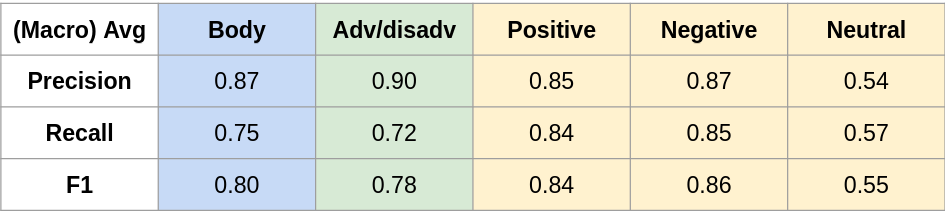
\includegraphics[width=15cm]{figs/fake.png}
\label{fig:test}
\end{figure}



\قسمت{دقت ‌مدل بر اساس معیارهای متفاوت روی شاخص گارانتی}

\begin{figure}[H]
\centering
\caption{ ‌مدل بر اساس معیارهای متفاوت روی شاخص گارانتی}\label{}
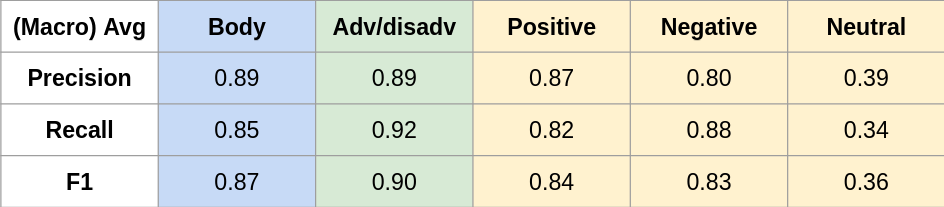
\includegraphics[width=15cm]{figs/warranty.png}
\label{fig:test}
\end{figure}


\قسمت{دقت ‌مدل بر اساس معیارهای متفاوت روی شاخص ابعاد}

\begin{figure}[H]
\centering
\caption{ ‌مدل بر اساس معیارهای متفاوت روی شاخص ابعاد}\label{}
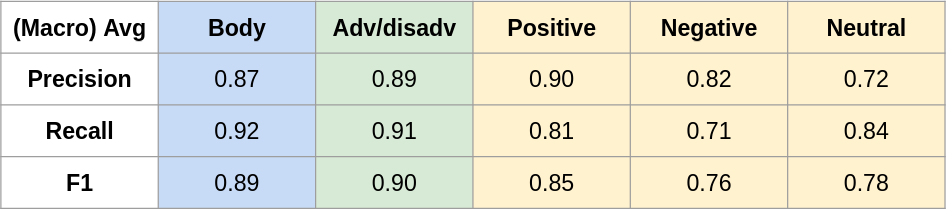
\includegraphics[width=15cm]{figs/size.png}
\label{fig:test}
\end{figure}



\قسمت{دقت ‌مدل بر اساس معیارهای متفاوت روی شاخص مغایرت کالا با کالای خریداری شده}

\begin{figure}[H]
\centering
\caption{ ‌مدل بر اساس معیارهای متفاوت روی شاخص مغایرت کالا با کالای خریداری شده}\label{}
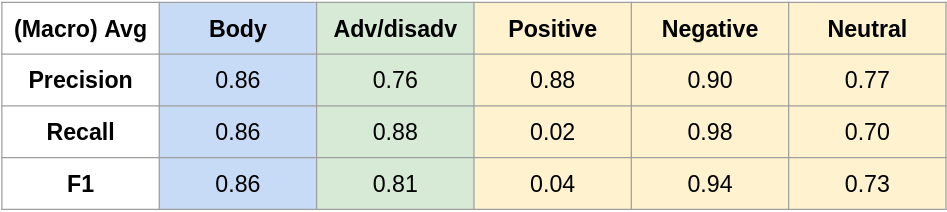
\includegraphics[width=15cm]{figs/discrepcency.png}
\label{fig:test}
\end{figure}


\قسمت{دقت ‌مدل بر اساس معیارهای متفاوت روی شاخص رایحه/بو}

\begin{figure}[H]
\centering
\caption{ ‌مدل بر اساس معیارهای متفاوت روی شاخص رایحه/بو}\label{}
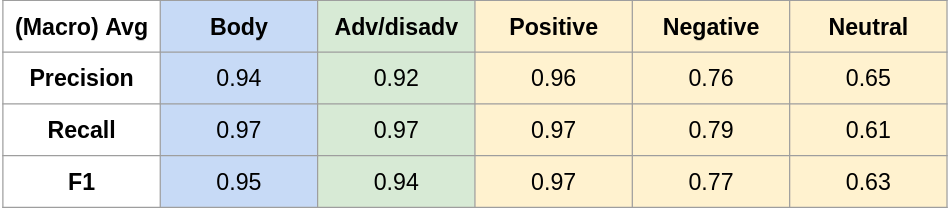
\includegraphics[width=15cm]{figs/flavor.png}
\label{fig:test}
\end{figure}



\قسمت{دقت ‌مدل بر اساس معیارهای متفاوت روی شاخص تاریخ انقضا}

\begin{figure}[H]
\centering
\caption{ ‌مدل بر اساس معیارهای متفاوت روی شاخص تاریخ انقضا}\label{}
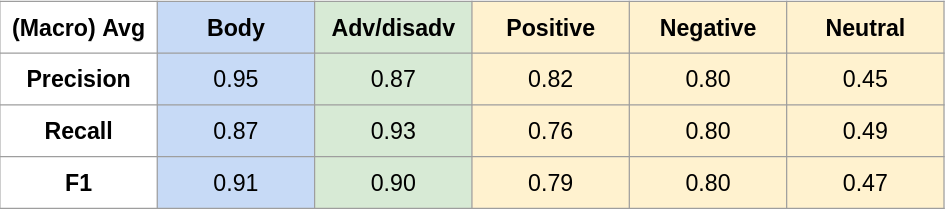
\includegraphics[width=15cm]{figs/expire.png}
\label{fig:test}
\end{figure}


\قسمت{جمع‌بندی}

با توجه به نتایج به دست آمده که آن‌ها را به‌طور دقیق در شکل‌ها بررسی نمودیم و با توجه به بالا بودن مقدار دقت با استفاده از تابع‌های هزینه‌ی 
\lr{Precision}
،
\lr{Recall}
و 
\lr{F1}
متوجه می‌شویم که مدل خروجی بسیار خوبی و مورد انتظاری دارد. لذا تنها کار برای پیش‌رفت مدل، جامع و مانع کردن آن می‌باشد که در بخش نتیجه‌گیری به‌طور کامل بدان می‌پردازیم.